\documentclass[xcolor={svgnames},aspectratio=169]{beamer}
% \usepackage[svgnames]{xcolor} % Must pass direct to beamer class
\usepackage[english]{babel}
\usepackage{lmodern}
\usepackage{libertinus}
\usepackage{csquotes}
\usepackage{multicol}
\usepackage{caption}
\usepackage{subcaption}
\usepackage{algorithm}
\usepackage{algpseudocode}
\usepackage{comment}
\usepackage{tikz}
    \usetikzlibrary{automata, positioning, calc}
    \usepackage{standalone} % Needed for Tikzscale
    \usepackage{tikzscale}  % Allows you to import and scale tikz like graphic
\usepackage{booktabs}

\usepackage{graphicx}
\makeatletter
\def\input@path{{Chapters/}{other/}{Figures/}{Tables/}}
\makeatother
\graphicspath{{Figures/}{Figures/Intro}{Figures/C1}{Figures/C2}{Figures/C3}}
\usepackage[backend=biber,style=authortitle,defernumbers=true]{biblatex} %authortitle authoryear ieee
% \usepackage[backend=biber,style=authoryear, citestyle=authoryear]{biblatex}
\addbibresource{../2025Bibs/Prospectus.bib}

\usepackage{xpatch}
\xapptobibmacro{cite}{\setunit{\nametitledelim}\printfield{year}}{}{}

\makeatletter
\renewrobustcmd{\blx@mkbibfootnote}[2]{%
  \iftoggle{blx@footnote}
    {\blx@warning{Nested notes}%
     \addspace\mkbibparens{#2}}
    {\unspace
     \ifnum\blx@notetype=\tw@
       \expandafter\@firstoftwo
     \else
       \expandafter\@secondoftwo
     \fi
       {\csuse{blx@theendnote#1}{\protecting{\blxmkbibnote{end}{#2}}}}
       {\csuse{footnote}[frame]{\protecting{\blxmkbibnote{foot}{#2}}}}}}
\makeatother




\title{Working Title}
% \subtitle{A Prospectus Defense}
\author{Capt. Brandon Hosley\inst{1}}
\institute[ENS]{
    \inst{1}
    Department of Operational Sciences\\
    Air Force Institute of Technology}
\date{\today}

\titlegraphic{
    \includegraphics[width=2cm]{afit_logo.png} \hfill
    \includegraphics[width=2cm]{en_logo.png}} 

\AtBeginSection[]{
  \begin{frame}
    \tableofcontents[currentsection, hideothersubsections]
  \end{frame}
}
\AtBeginSubsection[]{
  \begin{frame}
    \tableofcontents[currentsection, currentsubsection,
        subsectionstyle=show/shaded/hide, subsubsectionstyle=hide]
  \end{frame}
}

\usetheme{Montpellier}
\usecolortheme{orchid}
\mode<presentation>

\begin{document}

\frame{\titlepage}
\begin{frame}
    \tableofcontents[subsectionstyle=hide, subsubsectionstyle=hide]
\end{frame}

\section{Introduction}

\begin{frame}{The Vision for Autonomy in Defense}
    \begin{columns}
        \begin{column}{0.6\textwidth}
            \begin{itemize}
                \item \textbf{Department of Defense initiatives are actively advancing 
                    autonomous system deployment.}
                \begin{itemize}
                    \item \textbf{Replicator Initiative:} {Calls for the rapid integration of 
                        commercial-off-the-shelf (COTS) autonomous systems for scalable 
                        deployment. \footcite{robertson2023} }
                    \item \textbf{DARPA's OFFSET:} {Demonstrated feasibility of swarm-enabled 
                        ground and aerial assets in contested environments. 
                        \footcite{zotero-2835} }
                \end{itemize}
                \item \textbf{Limitation:} {Reliable autonomy in unpredictable environments 
                    remains an unsolved challenge.}
            \end{itemize}
        \end{column}
        \begin{column}{0.4\textwidth}
            \begin{figure}[!h]
                \centering
                \includegraphics[width=0.95\textwidth]{replicator_collage.png}
                \caption{\textbf{Replicator Initiative} aimed at multiple platforms. 
                    \footcite{robertson2023} }
                \label{fig:replicator_collage}
            \end{figure}
        \end{column}
    \end{columns}
\end{frame}


\begin{frame}{Rules-Based Control}
    \begin{columns}
        \begin{column}{0.6\textwidth}
            \begin{itemize}
                \item The earliest autonomous systems operate on hand-coded rules.
                \item Effective in constrained environments with predictable dynamics.
                \item Limitations:
                \begin{itemize}
                    \item Brittle under changing conditions.
                    \item Poor generalization to novel scenarios.
                \end{itemize}
                % \item Led to interest in adaptive learning systems.
            \end{itemize}
        \end{column}
        \begin{column}{0.4\textwidth}
            % \item Example is also the majority of video game "AI"
            \textbf{Example:}
            MYCIN, an expert System for diagnosis of bacterial infections \footcite{buchanan1984}.
            \begin{figure}[!h]
                \centering
                \includegraphics[width=0.65\textwidth]{mycin_logic.png}
                \caption{\textbf{MYCIN}'s logical flow.}
                \label{fig:mycin_logic}
            \end{figure}
        \end{column}
    \end{columns}
\end{frame}

\begin{frame}{Reinforcement Learning (RL)}
    \begin{itemize}
        \item RL enables agents to learn behaviors through trial and 
            error in dynamic environments.
        % \item Successes in single-agent settings with clear reward signals and isolated tasks.
    \end{itemize}
    \begin{columns}
        \begin{column}{0.65\textwidth}
            \begin{itemize}
                \item Generally follows the Agent-Environment Cycle (AEC) paradigm. 
                    \footcite{sutton2018}
                \begin{itemize}
                    \item Modeled well by Markov Decision Processes (MDPs).
                \end{itemize}
                \item Limitations:
                \begin{itemize}
                    \item Multi-agent scenarios are modeled by 
                        composed action and observation spaces.
                    \item Composed spaces are larger and encode more rigid agent interactions.
                \end{itemize}
            \end{itemize}
        \end{column}
        \begin{column}{0.3\textwidth}
            \begin{figure}[!h]
                \centering
                % 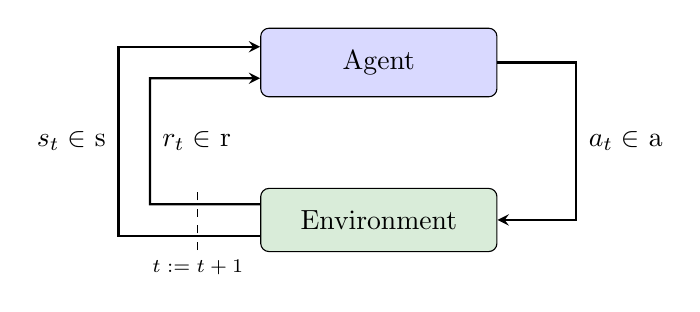
\begin{tikzpicture}[>=stealth, node distance=1cm, on grid, auto,
    entry/.style = {draw, rectangle, inner sep=8pt, rounded corners=3pt,
                    minimum width=3cm},
    arrow/.style = {thick,-stealth}]

    % States
    \node [] (center) {};
    \node [entry, fill= Blue!15] (agent) [above=of center] {Agent};
    \node [entry, fill=Green!15] (env) [below=of center] {Environment};
    \node [] (time) [below left= 0.6cm and 2.3cm of env]{\scriptsize\(t:=t+1\)};
    \draw [dashed] (time) -- +(0,1);

    % Transitions
    \draw [arrow] (agent.east) -- +(1,0) --coordinate(A) +(1,-2) -- (env.east);
    \draw [arrow] ([yshift=-0.2cm]env.west) -- +(-1.8,0) --coordinate(S) 
                    +(-1.8,2.4) -- ([yshift=+0.2cm]agent.west);
    \draw [arrow] ([yshift=+0.2cm]env.west) -- +(-1.4,0) --coordinate(R) 
                    +(-1.4,1.6) -- ([yshift=-0.2cm]agent.west);

    % Labels
    \node [] () [right= 1pt of A] {\(a_t\in\) \Gls{a}};
    \node [] () [left=  1pt of S] {\(s_t\in\) \Gls{s}};
    \node [] () [right= 1pt of R] {\(r_t\in\) \Gls{r}};
\end{tikzpicture}
                \includegraphics[width=0.95\textwidth]{ae_cycle.tex}
                \caption{\textbf{AEC}: Agent-Environment Cycle}
                \label{fig:ae_cycle}
            \end{figure}
        \end{column}
    \end{columns}
    % Extending Markov Chains (MDPs) to dynamic decision making
\end{frame}

\begin{frame}{Multi-Agent RL (MARL)}
    \begin{itemize}
        \item MARL extends RL to scenarios involving multiple learning agents.
        \item Used for both cooperative and competitive environments (e.g., games, simulations).
        \item Limitations:
        \begin{itemize}
            \item Often assumes agents are homogeneous or interchangeable.
            \item High coordination cost and non-stationarity challenges. \footcite{albrecht2024}
        \end{itemize}
    \end{itemize}
    \begin{figure}[!h]
        \centering
        \includegraphics[width=0.45\textwidth]{mae_cycle.tex}
        \caption{Multi-Agent AEC}
        \label{fig:marl_aec}
    \end{figure}
\end{frame}

\begin{frame}{Heterogeneous-Agent RL (HARL)}
    \begin{itemize}
        \item HARL addresses coordination among agents that may differ structurally in
            observation and/or action spaces.
    \end{itemize}
    \begin{columns}
        \begin{column}{.35\textwidth}
            \begin{itemize}
                \item Promising for real-world applications with diverse platforms 
                    (e.g., COTS drones, mixed teams\footcite{guo2024}).
                \item Limitations:
                \begin{itemize}
                    \item Limited literature.
                    \item Higher training cost than MARL.
                \end{itemize}
            \end{itemize}
            \hfil
        \end{column}
        \begin{column}{.6\textwidth}
            \begin{figure}[!h]
                \centering
                \includegraphics[width=0.75\textwidth]{hae_cycle.tex}
                \caption{Heterogeneous-Agent AEC}
                \label{fig:harl_aec}
            \end{figure}
        \end{column}
    \end{columns}
\end{frame}

\begin{frame}{Open Challenges in Scalable Multi-Agent Autonomy}
    \begin{itemize}
        \item Integration across heterogeneous platforms is constrained by inflexible model assumptions.
        \item Retraining cost grows rapidly with team size and complexity.
        \item Teams struggle to adapt dynamically to changing sensors or agent availability.
        \item Existing strategies for curriculum learning and network scaling are underdeveloped.
    \end{itemize}
\end{frame}

\begin{frame}{Why Heterogeneous Autonomy Matters}
\begin{columns}
    \begin{column}{0.6\textwidth}
    \begin{itemize}
        \item \textbf{Operational autonomy must account for platform diversity.}
        \begin{itemize}
            \item Teams may integrate UAVs and UGVs with different sensors, dynamics, and connectivity constraints.
            \item Heterogeneous-agent reinforcement learning (HARL) enables coordination across dissimilar platforms.
        \end{itemize}
        \item \textbf{Policy transfer and input-invariant networks} can support:
        \begin{itemize}
            \item Adaptability to new team compositions.
            \item Resilience to partial observation loss or sensor degradation.
        \end{itemize}
    \end{itemize}
    \end{column}
    \begin{column}{0.4\textwidth}
        \begin{figure}[!h]
            \centering
            \includegraphics[width=0.95\textwidth]{offset_collage.jpg}
            \caption{\textbf{OFFSET} test platforms.
                \footnote[frame]{\cite{zotero-2835}}}
            \label{fig:offset_collage}
        \end{figure}
    \end{column}
\end{columns}
\end{frame}

% Research Contributions
\begin{frame}{Research Contributions}
    \begin{itemize}
        \item {% Through-line:
            Advance the study of heterogeneous-agent reinforcement learning by exploring 
            scalable training architectures and policy designs that support adaptability 
            to agent diversity and team variation.}
            \begin{enumerate}
                \item {% Contribution 1:
                    Evaluate a policy upsampling strategy for training larger multi-agent teams 
                    more efficiently using pretrained smaller-team policies.}
                \item {% {Contribution 2:
                    Investigate input-invariant policy architectures for shared learning and 
                    robustness in teams of heterogeneous agents.}
                \item {% Contribution 3: 
                    Design and evaluate a curriculum that progressively expands network capacity 
                    via tensor projection to improve training efficiency.}
            \end{enumerate}
    \end{itemize}
\end{frame}

\begin{frame}{Research Objectives}
    \textbf{Contribution 1}
    % \textbf{Contribution 1 - Direct Scaling of Teams}
    \begin{itemize}
        \item {Improve training efficiency by scaling teams from smaller pretrained groups 
            using policy duplication instead of retraining from scratch.}
        \item {Demonstrate that policy reuse across increasing agent counts can reduce 
            training cost while maintaining performance.}
    \end{itemize}
    \vspace{1em}
    \textbf{Contribution 2}
    % \textbf{Contribution 2 - Input-Invariant Policy Architectures}
    \begin{itemize}
        \item {Construct input-invariant policy architectures to enable shared training 
            updates across agents with heterogeneous observation structures.}
        \item {Evaluate the effectiveness of input-invariant models in improving learning 
            efficiency in teams with overlapping observations.}
        \item {Test whether these models maintain stable performance under dynamic 
            observation space changes during execution.}
    \end{itemize}
\end{frame}

\begin{frame}{Research Objectives}
    \textbf{Contribution 3}
    % \textbf{Contribution 3 - Progressive Network Growth via Tensor Projections}
    \begin{itemize}
        \item {Demonstrate the feasibility of expanding a policy network mid-training 
            using tensor projection without discarding prior knowledge.}
        \item {Identify when during training such growth provides learning advantages 
            over fixed-size architectures.}
        \item {Compare performance and efficiency of progressive-growth networks to 
            fixed-size baselines in terms of convergence and cost.}
    \end{itemize}
\end{frame}


\section{Contribution 1}

% For each Contribution:
% Re-motiviate
%     Introduction
%         Lit review
%         Contribution
%     Methodology
%     Experimental Procedure
%     Results
%     Discussion

\subsection{Introduction}

\begin{frame}
\end{frame}

\subsubsection{Literature Review}

\subsubsection{Research Questions}

\begin{frame}{Research Questions}
    \begin{enumerate}
        \item[RQ 1] {
            Can pretraining smaller teams of agents and then scaling to the target 
            team size via policy duplication and retraining improve training efficiency 
            without sacrificing final policy performance in MARL?}
        \item[RQ 2] {
            How does the effectiveness of this direct scaling strategy vary across 
            environments with different forms of agent heterogeneity 
            (e.g., behavioral vs. intrinsic)?}
    \end{enumerate}
\end{frame}

\begin{frame}{RQ 1 - Research Tasks}
    \begin{enumerate}
        \item[RQ 1] \textcolor{gray}{
            Can pretraining smaller teams of agents and then scaling to the target 
            team size via policy duplication and retraining improve training efficiency 
            without sacrificing final policy performance in HARL? } \vspace{1em}
    \begin{itemize}
        \item[RT 1.1] {
            Design an upsampling-based curriculum using policy duplication and retraining.}
        \item[RT 1.2] {
            Define a metric (agent-steps) accounting for agent count and training time.}
        \item[RT 1.3] {
            Train tabula rasa agents each target environment and team size as baselines.}
        \item[RT 1.4] {
            Evaluate training performance across various pretraining length and target team sizes.}
    \end{itemize}
    \end{enumerate}
\end{frame}

\begin{frame}{RQ 2 - Research Tasks}
    \begin{enumerate}
        \item[RQ 2] \textcolor{gray}{
            How does the effectiveness of this direct scaling strategy vary across 
            environments with different forms of agent heterogeneity 
            (e.g., behavioral vs. intrinsic)? } \vspace{1em}
    \begin{itemize}
        \item[RT 2.1] {
            Select environments that represent distinct forms of agent heterogeneity. \\
            Behavioral, Intrinsic.}
        \item[RT 2.2] {
            Adapt observation structures to enable fixed policy architectures across team sizes.}
        \item[RT 2.3] {
            Evaluate the effect of heterogeneity type on the scalability and retraining benefit.}
    \end{itemize}
    \end{enumerate}
\end{frame}

% \subsection{Methodology}
% \subsection{Experimental Procedure}
% \subsection{Results}
% \subsection{Discussion}
\section{Contribution 2}

% For each Contribution:
%     Introduction
%         Recall Motivation
%         Lit review
%         Contribution
%     Methodology
%     Experimental Procedure
%     Results
%     Discussion

\subsection{Introduction}

\begin{frame}{The Case for Input-Invariant Architectures}
    \begin{itemize}
        \item Heterogeneous agent teams frequently encounter differences in observation 
            structure due to varying sensor suites and mission roles.
        \item Traditional policy networks require fixed, consistent inputs—limiting their 
            ability to scale or adapt.
        \item Input-invariant architectures offer a promising alternative by allowing 
            policies to generalize across agents and configurations without retraining.
        \item This contribution explores how these architectures can improve learning 
            efficiency and robustness in dynamic, real-world team settings.
    \end{itemize}
\end{frame}

\subsubsection{Literature Review}


% #TODO: Pull from Paper Draft


\subsubsection{Research Questions}

\begin{frame}{Contribution 2 - Research Questions}
    \begin{enumerate}
        \item[RQ 1] {
            How does incorporating input-invariant structures \emph{(i.e., networks 
            that are robust to feature permutation and input length differences)}
            into policy networks affect learning efficiency and team robustness 
            when heterogeneous agents have partially overlapping observations?
            }
        \item[RQ 2] {
            Do input-invariant architectures lead to more stable policy performance under 
            team-size changes and partial observation loss during execution?
            }
    \end{enumerate}
\end{frame}

\begin{frame}{RQ 1 - Research Tasks}
    \begin{enumerate}
        \item[RQ 1] \textcolor{gray}{
            How does incorporating input-invariant structures \emph{(i.e., networks 
            that are robust to feature permutation and input length differences)}
            into policy networks affect learning efficiency and team robustness 
            when heterogeneous agents have partially overlapping observations? } \vspace{1em}
    \begin{itemize}
        \item[RT 1.1] {
            Design and implement a policy architecture that exhibits input-invariance through 
            techniques such as pooling layers, attention mechanisms, or permutation-invariant 
            encodings.}
        \item[RT 1.2] {
            Identify benchmark environments where agents possess distinct but partially 
            overlapping observation features (e.g., different sensor arrays).}
        \item[RT 1.3] {
            Train these, input-invariant policy networks in the selected setting(s) and measure 
            learning rate and convergence behavior.}
        \item[RT 1.4] {
            Compare input-invariant shared architectures against baseline (non-invariant) 
            architecture to evaluate performance and learning benefits.}
    \end{itemize}
    \end{enumerate}
\end{frame}

\begin{frame}{RQ 2 - Research Tasks}
    \begin{enumerate}
        \item[RQ 2] \textcolor{gray}{
            Do input-invariant architectures lead to more stable policy performance under 
            team-size changes and partial observation loss during execution? } \vspace{1em}
    \begin{itemize}
        \item[RT 2.1] {
            Simulate runtime degradation by selectively masking subsets of agent observations 
            (e.g., sensor failure) for both the input-invariant and baseline policy models.}
        \item[RT 2.2] {
            Simulate dynamic changes in team size by removing agents during evaluation 
            in both the input-invariant and baseline policy models.}
        \item[RT 2.3] {
            Measure policy stability, reward degradation, and recovery behavior under these 
            perturbations for both the input-invariant and baseline models.}
        \item[RT 2.4] {
            Statistically compare performance between input-invariant and baseline models 
            across all perturbation conditions to assess resilience and stability.}
    \end{itemize}
    \end{enumerate}
\end{frame}


% \subsection{Methodology}



\subsection{Environment Model}


% \subsection{Experimental Procedure}
% \subsection{Results}
% \subsection{Discussion}


\section{Contribution 3}

% For each Contribution:
%     Introduction
%         Recall Motivation
%         Lit review
%         Contribution
%     Methodology
%     Experimental Procedure
%     Results
%     Discussion
\subsection{Introduction}

\subsubsection{Literature Review}

\subsubsection{Research Questions}

\begin{frame}{Contribution 3 - Research Questions}
    \begin{enumerate}
        \item[RQ 1] {
            To what (if any) extent do graph-based policies improve learning efficiency 
            in heterogeneous-agent environments compared to other architectures?
            }
        \item[RQ 2] {
            How robust are graph-based policies to perturbations such as changes to 
            partial observability and changes in team composition?
            }
        \item[RQ 3] {
            What are the computational and implementation costs of graph-based 
            architectures relative to their performance benefits?
            }
    \end{enumerate}
\end{frame}

\begin{frame}{RQ 1 - Research Tasks}
    \begin{enumerate}
        \item[RQ 1] \textcolor{gray}{ 
            To what (if any) extent do graph-based policies improve learning efficiency 
            in heterogeneous-agent environments compared to other architectures? } \vspace{1em}
    \begin{itemize}
        \item[RT 1.1] {
            Implement and train a graph-based architecture such as 
            PIC in the custom heterogeneous environment.}
        \item[RT 1.2] {
            Measure convergence rates and final performance across 
            multiple team compositions and sizes.}
        \item[RT 1.3] {
            Compare against performance of input-invariant and 
            non-shared baselines (from Contribution 2).}
    \end{itemize}
    \end{enumerate}
\end{frame}

\begin{frame}{RQ 2 - Research Tasks}
    \begin{enumerate}
        \item[RQ 2] \textcolor{gray}{ 
            How robust are graph-based policies to perturbations such as changes to 
            partial observability and changes in team composition? } \vspace{1em}
    \begin{itemize}
        \item[RT 2.1] {
            Evaluate robustness to agent dropout and team-size changes at test time.}
        \item[RT 2.2] {
            Introduce random observation channel masking and measure recovery/stability.}
        \item[RT 2.3] {
            Compare perturbation response curves with Contribution 2 architectures.}
    \end{itemize}
    \end{enumerate}
\end{frame}

\begin{frame}{RQ 3 - Research Tasks}
    \begin{enumerate}
        \item[RQ 3] \textcolor{gray}{ 
            What are the computational and implementation costs of graph-based 
            architectures relative to their performance benefits? }
        \vspace{1em}
        \begin{itemize}
            \item[RT 3.1] {
                Benchmark computational cost during training and 
                inference (e.g., agent-steps, step-costs).}
            \item[RT 3.2] {
                Perform Statistical comparison of relative training cost, rate of convergence, 
                in training and rate of performance degradation in completed models.}
        \end{itemize}
    \end{enumerate}
\end{frame}







\subsubsection{Training Architectures}

\begin{frame}{Architectures Compared (RT 1.1,1.4)}
    \textbf{Models Evaluated}
    \begin{enumerate}
        \item \textbf{HAPPO (Baseline)}\footcite{zhong2024} As used in Contribution 2
        \item \textbf{Mean-Field } From Contribution 2
        \item \textbf{PIC}\footcite{liu2020b}
          \begin{itemize}
            % \item \emph{COMA + GNN + Transformer}
            \item \emph{GNN + MADDPG}
            \item Graph neural network for relational encoding.
            \item Transformer-based critic for contextual estimation.
            \item Chosen due to its conceptual similarity to the author's own attempted 
                implementation of a minimal GNN-based MARL architecture:
            \begin{itemize}
                \item Efforts to independently develop a simple graph-based model yielded architecture nearly equivalent to PIC.
                \item Provides a representative implementation for graph-based learning in MARL under heterogeneous conditions.
                \item Well-established architecture that integrates GNN message passing and attention mechanisms in a scalable way.
            \end{itemize}
          \end{itemize}
    \end{enumerate}
\end{frame}


% \subsection{Methodology}
% \subsection{Experimental Procedure}
% \subsection{Results}
% \subsection{Discussion}

% Prospectus, schedule

\section{Conclusion}

\begin{frame}
    \centering
    \Huge
    Questions?
\end{frame}

\section{References}

% \nocite{*}
\renewcommand*{\bibfont}{\tiny}
\frame[allowframebreaks]{\printbibliography}

\end{document}
